\textcolor{black}{\section{Procedimiento}}
Para determinar la relación carga eléctrica del electrón con la constante de Boltzmann se utilizo la ecuación Shockley para polarización directa al desarrollar la  ecuación (\ref{Shockley1}) cuando $I_d >> I_s$ obtenemos:
\begin{equation}
	I_d \approx I_s \exp\left(\frac{eV_d}{nk_b T}\right)
	\label{shock2}
\end{equation}
Al aplicar el logaritmo a ambos lados se ajusta linealmente, la pendiente del ajuste nos muestra la relación $e/k_b$:
\begin{equation}
	\underbrace{\ln(I_d)}_{y} = \underbrace{\frac{e}{nk_b T}}_{m} \cdot \underbrace{V_d}_{x}  + \underbrace{ln(I_s)}_{b}
	\label{shock3}
\end{equation}

Una vez obtenida la relación lineal, se procedió a obtener la dupla de datos ($V_d, I_d$) de manera experimental para esto se utilizó un modulo M05, que tienen un circuito eléctrico interno como el que se muestra en la figura (\ref{Circuito M05}) 
\begin{figure}[htpb]
	\centering
	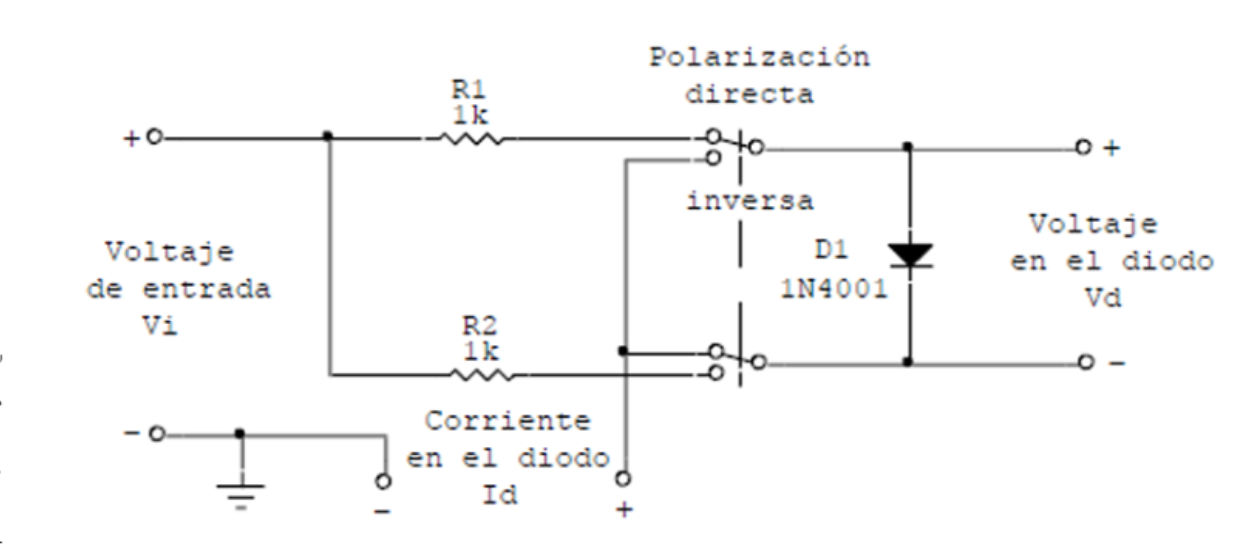
\includegraphics[scale=0.35]{figs/M05.png}
	\caption{Circuito eléctrico interno del modulo M05}
	\label{Circuito M05}
\end{figure}
Primero se conecto la fuente de voltaje de una consola LEB01 a la entrada 1 de la misma, luego para alimentar el módulo M05 este se conecto a el puerto 5 de la consola, proporcionando el voltaje de polarización. Después se conecto un multímetro en paralelo a los puertos del modulo para medir la caída de tensión $V_d$ en el diodo, así como también se conecto otro multímetro en serie con el circuito, utilizando las salidas 1 y 2 de la consola para medir la corriente directa $I_d$, el arreglo final se muestra en la figura (\ref{Conexion})
\begin{figure}[htpb]
	\centering
	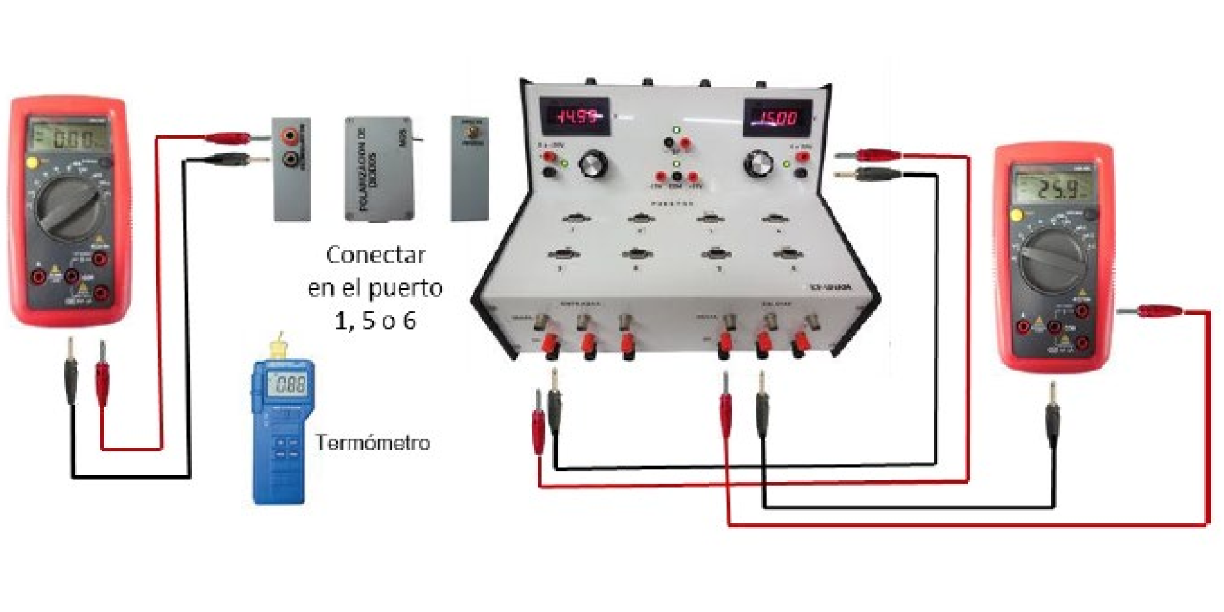
\includegraphics[scale=0.35]{figs/Conexion.png}
	\caption{Esquema de conexión}
	\label{Conexion}
\end{figure}
\FloatBarrier
Una vez verificado el montaje, se coloco el Modulo M05 en polarización directa y se fue suministrando un voltaje de entrada ($V_i$) de 0 a 15V en pasos de 0.2V registrando para cada paso los valores de corriente $I_d$ y voltaje $V_d$. A continuación se repitió el procedimiento pero esta vez colocando el modulo M05 en polarización inversa. 
Finalmente, se midió la temperatura ambiente con un termómetro. 
\noindent 